\documentclass[journal]{IEEEtran}

% ===== XeLaTeX / Unicode 字体路线 =====
\usepackage{iftex}
\ifXeTeX
  \usepackage{fontspec}
  \usepackage{xeCJK}
  \usepackage{amsmath}
  \usepackage{unicode-math}
  \usepackage{algorithm}
  \usepackage{algorithmic}

  % 关键：延后覆盖 IEEEtran 的 ptm 设置，避免 TU/ptm 报错
  \AtBeginDocument{%
    % 正文字体
    \setmainfont{TeX Gyre Termes}
    \setsansfont{TeX Gyre Heros}
    \setmonofont{JetBrains Mono}
    \setCJKmainfont{Noto Serif CJK SC}[BoldFont=Noto Serif CJK SC]

    % 数学字体
    \setmathfont{TeX Gyre Termes Math}
  }
\else
  % 如果不是 XeLaTeX（比如 pdfLaTeX），这里可以放兼容方案或直接报错
\fi

% ===== 常用宏包 =====
\usepackage{graphicx}
\usepackage{booktabs}
\usepackage{threeparttable}
\usepackage{float}
\usepackage{cite}

\begin{document}
\title{From Noisy Conflict Scores to Forecastable Risk States in Social Media Comment Streams}

\author{Linli~Zhu\ (朱林立)\IEEEauthorrefmark{1}, Ziqiang~Ma\ (马自强)\IEEEauthorrefmark{2}%
\thanks{Manuscript received Month DD, YYYY; revised Month DD, YYYY.}%
\thanks{\IEEEauthorrefmark{1}L. Zhu is with the School of Computer Science, Ningxia University, Yinchuan, China (e-mail: violina2333@gmail.com). Code: https://github.com/Megalomanian/conflict-early-warning.}%
\thanks{\IEEEauthorrefmark{2}Z. Ma is with the School of Information Engineering, Ningxia University, Yinchuan, China (e-mail: maziqiang@nxu.edu.cn). Corresponding author.}}

\maketitle

\begin{abstract}
Social media conflict forecasting promises earlier intervention than post-hoc content classification, yet raw text-derived scores are sparse and temporally noisy. We construct a conflict index without task-specific labels and introduce a leakage-resistant cleaning pipeline that regularizes the 12-hour time axis, learns all calibration and cleaning statistics from training data only, and performs causal exponential smoothing. A logistic model predicts whether the stabilized state will exceed the topic-specific training-period 80th percentile within the next six bins. Smoothing, regularization, decision threshold, and feature-set complexity are selected on validation data; the final 25\% of each topic is held out for testing. The validation rule selects a parsimonious state-history model. Across 20 Zhihu topics and 1,706 test windows, it achieves AUC $0.891$, precision $0.738$, recall $0.822$, and F1 $0.778$, compared with persistence recall $0.584$ and F1 $0.716$. Topic-level paired bootstrap confirms gains in F1 ($+0.062$, 95\% CI $[0.018,0.108]$) and recall ($+0.241$, $[0.173,0.317]$); F1 improves on 15 of 20 topics. Results remain positive at 70th, 80th, and 90th-percentile risk definitions. Continuous-value regression remains below persistence, showing that causal state modeling supports high-risk-state prediction but not exact trajectory forecasting.
\end{abstract}

\begin{IEEEkeywords}
conflict-index construction, data cleaning, causal smoothing, risk-state prediction, social media comments, temporal split
\end{IEEEkeywords}

\section{Introduction}

\subsection{Challenges in Governing Social Media Public Opinion}
The ubiquity of social media has transformed how information is produced, circulated, and contested. Public debates that once unfolded over days now escalate within hours as platforms enable rapid information cascades and viral diffusion~\cite{Vosoughi2018}. Seemingly marginal topics can ignite large-scale opinion swings with tangible offline consequences. For example, coordinated online discourse has been shown to correlate with mass protests and even violent incidents in subsequent days~\cite{Steinert2015,Arcila2024}.

\subsubsection{Information Cascades and Offline Spillovers}
Information spreads faster than it can be verified. Emotional contagion and algorithmic amplification jointly fuel cascades that can spill over into offline actions. Once critical mass is reached, moderation or fact-checking becomes less effective, as narratives solidify through repeated exposure~\cite{Vosoughi2018}. These cascades thus demand proactive, not reactive, management.

\subsubsection{Delays in Post-hoc Sentiment Analysis}
Conventional sentiment analysis frameworks primarily offer retrospective insight: they describe how people felt after events unfolded. However, by the time significant polarity shifts are detected, the discussion may already have escalated beyond control. This latency between event occurrence and analytical response undermines the capacity for early intervention~\cite{Wang2020}.

\subsubsection{Research Gaps in Early Warning}
Despite advances in opinion mining and social listening, few studies explicitly target early warning. Existing tools classify emotions or toxicity per message, but rarely attempt to forecast when online discontent is likely to escalate~\cite{Wang2020}. This absence of anticipatory modeling creates a crucial gap between detection and prevention. At the same time, converting a post-level score into a forecast target introduces an often overlooked assumption: the aggregated semantic signal must exhibit stable temporal dependence. A forecasting model cannot recover predictive structure that is absent from its input trajectory.

\subsection{Limitations of Existing Technical Paradigms}

\subsubsection{Lexicon/Rule-Based Systems: Cross-Language and Sarcasm Fragility}
Lexicon-based or rule-driven systems offer interpretability but struggle with context-dependent semantics, sarcasm, and multilingual variation. Irony (“Great, another perfect policy!”) or cultural idioms can easily invert meaning~\cite{Dhumpati2025}. Moreover, such systems require language-specific dictionaries that fail in cross-lingual or code-mixed environments~\cite{Kaity2020}.

\subsubsection{Static Classifiers: Concept Drift and Out-of-Distribution Failure}
Traditional supervised classifiers, like \emph{SVM} or \emph{CNN}, are trained on fixed datasets and assume distributional stability. In dynamic online environments, vocabulary, sentiment norms, and social topics evolve rapidly—an issue known as concept drift~\cite{Gama2014}. Without continuous adaptation, static models degrade, misclassify emergent patterns, or fail to generalize to unseen contexts.

\subsubsection{Post-Level Semantic Analysis without Temporal Escalation Modeling}
Recent pretrained language models and text analysis systems substantially improve post-level semantic understanding, sentiment recognition, and harmful-content detection. However, these methods are often used to score or classify comments independently, without explicitly modeling how conflict accumulates and evolves across time. Consequently, they provide informative local signals but limited support for topic-level escalation forecasting and early warning. This motivates the introduction of a temporal forecasting layer on top of interpretable post-level risk signals~\cite{Abdalgader2025}.

\subsection{Contributions of This Work}

To examine this assumption, we construct a conflict index without task-specific labels and evaluate when its resulting trajectories can and cannot be forecast by supervised temporal models. Rather than presenting a new neural architecture as the central contribution, we focus on signal stability, temporal dependence, and leakage-resistant evaluation. The main contributions are as follows:

\noindent\textbf{(I-C1) Conflict-index quantification framework (Sec.~III-B):}
We operationalize a candidate \emph{conflict index} by combining attack-related negativity, negative high-arousal emotion, and stance polarization into a unified post-level score without task-specific conflict labels. This unsupervised construction stage is distinct from the downstream forecasters, which are trained with historical trajectory targets.

\noindent\textbf{(I-C2) Causal signal cleaning and risk-state formulation (Sec.~\ref{sec:impl}):}
We regularize sparse topic streams on their true time axis, learn all clipping, imputation, scaling, and risk thresholds from training data only, and use causal smoothing to separate persistent risk states from bin-level semantic noise. Validation data select the smoothing scale and the smallest feature set within 0.005 F1 of the best candidate, without accessing the final test period.

\noindent\textbf{(I-C3) Positive real-data risk-state prediction with boundary analysis (Sec.~\ref{sec:discussion}):}
On held-out Zhihu periods, the selected state-history model improves F1 and recall over persistence across most topics, with paired topic-bootstrap intervals excluding zero. Threshold and feature ablations show that causal state history---rather than additional noisy semantic components---drives the gain. Exact-value regression remains persistence-dominated.

\subsection{Paper Structure Overview}
The remainder of this paper is organized as follows. Section~II reviews related studies in sentiment analysis, harmful content detection, and temporal modeling. Section~III presents conflict-index construction, signal cleaning, and the two temporal prediction tasks. Section~IV reports synthetic continuous forecasting, real-data risk-state prediction, boundary analysis, and limitations.

\section{Related Work}

\subsection{Deep Learning for Sentiment and Emotion Understanding}
Deep learning has significantly advanced sentiment analysis by learning contextual and compositional linguistic patterns that are difficult to encode with lexicon-based rules or handcrafted features. Recent surveys~\cite{birjali2021sentiment,wahid2025crisis} trace this evolution from classical approaches to neural architectures, highlighting how LSTMs, CNNs, and Transformer encoders (e.g., BERT and GPT-style models) improve classification accuracy through representation learning. Despite these gains, key challenges remain, including robustness to sarcasm and irony, domain shift across platforms and topics, multilingual and code-mixed text processing, and the need for explainable sentiment reasoning for high-stakes governance applications~\cite{birjali2021sentiment}. Recent work also moves beyond categorical sentiment labels toward continuous intensity scoring---for instance, SafeSpeech~\cite{ghosh2024safespeech} uses integrated gradients to assign fine-grained hate-intensity scores to individual words, enabling more nuanced risk assessment than binary classification. These limitations motivate models that (i) provide interpretable intermediate signals and (ii) remain effective under rapidly changing discourse.

\subsection{Risk Scoring for Harmful Content and Hazardous Conversations}
Beyond categorical sentiment labels, risk scoring aims to assign continuous severity estimates to online comments to support scalable moderation and hazard monitoring. Wulczyn \emph{et al.}~\cite{Wulczyn2017} construct a large corpus of Wikipedia discussion comments annotated for personal attacks and train predictive models that output, for each comment, the probability of being an attack. Such probabilistic outputs serve as practical risk scores for triage and prioritization, enabling moderators to focus on high-risk items and to identify discussion spaces with elevated aggression. However, most risk-scoring systems remain \emph{instance-centric}: they optimize snapshot detection at the comment level and treat posts as independent samples. As a result, they do not explicitly characterize how risk accumulates and propagates within a topic over time, nor do they naturally support trajectory-level forecasting and early warning. The conflict-index formulation in this paper builds on the idea of continuous risk scoring~\cite{ghosh2024safespeech} while explicitly designing the score to be both post-level interpretable and suitable as a temporal signal for escalation modeling.

\subsection{Temporal Forecasting of Public Opinion Trends with LSTM Variants}
Forecasting public opinion dynamics during emergencies requires temporal models that can capture persistence, volatility, and bursty surges in online activity. LSTM-based predictors are widely adopted for such sequence modeling, but their performance can be sensitive to hyperparameter choices under highly nonlinear and nonstationary trends. To improve forecasting stability, Mu \emph{et al.}~\cite{Mu2023IPSO} propose an Improved Particle Swarm Optimization LSTM (IPSO--LSTM) framework that uses adaptive search strategies (e.g., nonlinearly decreasing inertia weights and mutation mechanisms) to tune LSTM hyperparameters and avoid poor local optima. Their results show improved error metrics (e.g., MAPE and RMSE) relative to standard LSTM variants on multiple emergency-event datasets~\cite{Mu2023IPSO}. While these studies demonstrate the value of enhanced temporal predictors, they typically operate on aggregate time series and do not incorporate fine-grained, post-level semantic evidence. Our work complements this line of research by coupling contextual language understanding (via sentence-embedding-derived conflict signals) with temporal sequence modeling (via LSTM) to produce interpretable, topic-level escalation trajectories and short-horizon risk forecasts.

Recent hybrid architectures further validate the CNN-LSTM paradigm for social-media event forecasting. Singh and Jain~\cite{singh2025cupcdlstm} combine DistilBERT embeddings with CNN-LSTM layers to predict civil unrest events from Twitter data, demonstrating cross-region generalizability. Upadhyay \emph{et al.}~\cite{upadhyay2024satcobilstm} propose a self-attention BiLSTM with multi-scale CNN for crisis event detection, achieving strong F1 scores across benchmark datasets. On the theoretical side, Liu \emph{et al.}~\cite{liu2025memory} identify multi-scale memory cycles in public opinion time series, providing empirical support for the sliding-window formulation with carefully chosen lookback length $L$ and forecast horizon $H$. For crisis-specific forecasting, Lou \emph{et al.}~\cite{lou2024cnnlstm} demonstrate that CNN-LSTM hybrid architectures outperform standalone CNN, LSTM, and Transformer variants by 4--6\% on social-network crisis prediction tasks. We also note the emergence of efficient Transformer architectures for long-sequence forecasting, such as Informer~\cite{zhou2021informer}, which uses ProbSparse self-attention to achieve $O(L\log L)$ complexity; these methods are primarily designed for sequences with hundreds to thousands of time steps, whereas our setting involves relatively short lookback windows ($L{=}12$) where lightweight recurrent architectures remain competitive.

\subsection{Information Cascade and Diffusion Prediction}

Beyond post-level content analysis, modeling how information spreads through social networks is essential for understanding conflict escalation dynamics. Recent graph-based approaches have advanced cascade prediction: Xu \emph{et al.}~\cite{xu2025d2} propose D\textsuperscript{2}, a two-stage GNN framework that first predicts future propagation paths from limited early-stage data, then detects rumors via neural architecture search over the completed graph. The same group extends this to hypergraph neural networks, in HyperIDP~\cite{xu2025hyperidp}, jointly handling macroscopic cascade scale prediction and microscopic next-user forecasting with a cooperative-adversarial multi-task loss~\cite{xu2025hyperidpB}. These works highlight the value of modeling diffusion structure for early detection; our work complements them by focusing on \emph{content-driven} conflict signals rather than propagation topology, making the two approaches orthogonal and potentially synergistic.

\section{Conflict-Index Construction and Temporal Prediction}

\subsection{Problem Definition}

We study social-media comment streams organized by topic and discretized into fixed-length time bins. For a given topic, let the observation period be partitioned into $T$ consecutive bins of equal duration. For notation simplicity, we omit the topic index in the following definitions. Denote by $\mathcal{B}_t = \{x_{t,i}\}_{i=1}^{n_t}$ the multiset of $n_t$ comments posted in bin $t \in \{1, \dots, T\}$, where each $x_{t,i}$ represents a text message.

Our first objective is to assign an interpretable \emph{conflict index} to each comment via a text encoder $f_\theta$:
\begin{equation}
c_{t,i} = f_\theta(x_{t,i}) \in [0, 1],
\end{equation}
where higher values indicate stronger antagonistic cues (e.g., high-arousal negative emotion and confrontation markers). To obtain a topic-level risk signal per bin, we aggregate comment-level indices using a fixed aggregation operator $\mathrm{Agg}(\cdot)$:
\begin{equation}
\bar{c}_t = \mathrm{Agg}\left(\{c_{t,i}\}_{i=1}^{n_t}\right) \in [0, 1].
\end{equation}

Our second objective is to test whether this proxy is forecastable through short-horizon prediction. Given the historical binned sequence $\bar{c}_{1:t}$, we learn a temporal predictor $g_\phi$ to estimate the future trajectory $\mathbf{\hat{c}}$ over a horizon $H$:
\begin{equation}
\mathbf{\hat{c}}_{t+1:t+H} = g_\phi(\bar{c}_{1:t}).
\end{equation}
An escalation warning is triggered at time bin $t$ if the predicted risk is expected to exceed a predefined threshold $\eta$ within the horizon, i.e.,
\begin{equation}
\max_{1 \le h \le H} \hat{c}_{t+h} \ge \eta,
\end{equation}
optionally combined with a rapid-growth criterion to capture fast-rising trends.

\subsection{Conflict-Index Quantification without Manual Labels}\label{sec:conflict_index}

Our dataset contains only time-stamped comment text streams and provides no human-annotated conflict labels. We therefore construct a candidate unsupervised \emph{conflict index} by combining three interpretable proxies: (i) attack-related negativity, (ii) negative high-arousal emotion intensity, and (iii) stance polarization derived from within-bin semantic bimodality. Because these components are not validated against task-specific annotations, the resulting quantity is an operational proxy whose construct validity must be evaluated separately from its temporal predictability. For each comment $x_{t,i}$ posted in time bin $t$, we compute
\begin{equation}
c_{t,i} = \sigma\!\left(w_a \tilde{a}_{t,i} + w_e \tilde{e}_{t,i} + w_s \tilde{s}_{t,i} + b\right)\in[0,1],
\label{eq:conflict_index_fusion}
\end{equation}
where $\sigma(\cdot)$ is the sigmoid function, $w_a,w_e,w_s \ge 0$ control the relative contributions (e.g., $w_a:w_e:w_s = 0.5:0.3:0.2$), and $b$ is a bias term. The tildes denote \emph{distribution-calibrated} scores (Sec.~\ref{sec:calibration}) so that components from different sources become comparable.

\subsubsection{Attack/Antagonism Intensity from a Pretrained Harm Model}
We obtain an antagonism score from a pretrained harmful/attack detector (e.g., toxicity/insult/hate model) that outputs a probability of attack-like content for a given text:
\begin{equation}
a_{t,i} = h_{\psi}(x_{t,i}) \in [0,1],
\label{eq:attack_score}
\end{equation}
where $h_{\psi}$ is a frozen pretrained model. This score serves as a \emph{pseudo-label prior} capturing confrontation markers, threats, harassment, and abusive language without requiring any task-specific annotation.

\subsubsection{Emotion Intensity from a Zero-Shot Emotion Model}
We characterize emotionally charged negativity using a zero-shot (or pretrained) emotion model that produces probabilities for emotion categories. Let $p_{\text{neg}}(x_{t,i})$ denote the probability of negative sentiment and $p_{\text{anger}}(x_{t,i})$ denote the probability of anger (a high-arousal negative emotion). We define
\begin{equation}
e_{t,i} = \alpha\, p_{\text{neg}}(x_{t,i}) + (1-\alpha)\, p_{\text{anger}}(x_{t,i}), \quad \alpha \in [0,1],
\label{eq:emotion_score}
\end{equation}
where $\alpha$ balances general negativity and arousal-related anger (we use $\alpha\in[0.6,0.8]$ in practice). This construction rewards comments that are both negative and emotionally intense, which are common precursors to conflict escalation. Recent empirical evidence from Weibo conflict discourse networks confirms that emotional similarity (affective homophily)---rather than structural prestige---is the dominant organizing principle in online conflict, validating the central role of negative high-arousal emotion in our conflict-index formulation~\cite{gu2025affective}.

\subsubsection{Stance Polarization via Within-Bin Semantic Bimodality}
In the absence of stance labels (pro/con/neutral), we estimate polarization by measuring whether comments within the same time bin form two semantically separated camps---an unsupervised approach inspired by embedding-based stance detection methods~\cite{kucuk2020stance}. We first compute sentence embeddings using a frozen encoder $\mathrm{Enc}(\cdot)$ (e.g., multilingual BERT pooling or sentence-transformer):
\begin{equation}
\mathbf{v}_{t,i} = \mathrm{Enc}(x_{t,i}) \in \mathbb{R}^d.
\label{eq:embedding}
\end{equation}
Within bin $t$, we apply $k{=}2$ clustering (e.g., k-means) on $\{\mathbf{v}_{t,i}\}_{i=1}^{n_t}$ to obtain two cluster centroids $\mathbf{u}_{t,1}$ and $\mathbf{u}_{t,2}$. The inter-camp separation is measured by
\begin{equation}
\Delta_t = 1 - \cos(\mathbf{u}_{t,1}, \mathbf{u}_{t,2}) \in [0,2],
\label{eq:camp_separation}
\end{equation}
where $\cos(\cdot,\cdot)$ is cosine similarity. Next, we quantify how strongly each comment aligns with one camp over the other. Let $d(\cdot,\cdot)$ be a distance function (we use cosine distance). Define the camp-alignment confidence
\begin{equation}
q_{t,i} = \frac{\left|d(\mathbf{v}_{t,i},\mathbf{u}_{t,1}) - d(\mathbf{v}_{t,i},\mathbf{u}_{t,2})\right|}
{d(\mathbf{v}_{t,i},\mathbf{u}_{t,1}) + d(\mathbf{v}_{t,i},\mathbf{u}_{t,2}) + \epsilon} \in [0,1],
\label{eq:alignment_confidence}
\end{equation}
with a small $\epsilon>0$ to avoid division by zero. Finally, the stance polarization score for a comment is
\begin{equation}
s_{t,i} = \mathrm{norm}(\Delta_t)\cdot q_{t,i} \in [0,1],
\label{eq:stance_score}
\end{equation}
where $\mathrm{norm}(\Delta_t)$ maps the separation magnitude to $[0,1]$ (e.g., $\mathrm{norm}(\Delta_t)=\min(1,\Delta_t)$). This assigns higher polarization to bins that exhibit two distinct camps and to comments that are clearly affiliated with one camp. This unsupervised embedding-based approach to polarization measurement aligns with recent work on transformer-based echo chamber quantification~\cite{ghafouri2024echo} and unsupervised polarization knowledge extraction from text corpora~\cite{paschalides2025polar}.

\subsubsection{Distribution Calibration by Percentile Mapping}\label{sec:calibration}
Scores produced by different pretrained models and heuristics can have inconsistent scales and distributions. We therefore calibrate each raw component score using an empirical cumulative distribution function (ECDF) fitted only on comments in the temporal training segment of each topic. For a raw score $r_{t,i}\in[0,1]$ (standing for $a_{t,i}$, $e_{t,i}$, or $s_{t,i}$), we define
\begin{equation}
\tilde{r}_{t,i} = \mathrm{ECDF}_r(r_{t,i}) \in [0,1],
\label{eq:ecdf}
\end{equation}
which maps $r_{t,i}$ to its percentile rank. This calibration yields comparable $\tilde{a}_{t,i},\tilde{e}_{t,i},\tilde{s}_{t,i}$ for fusion in (\ref{eq:conflict_index_fusion}).

\subsubsection{Bin-Level Aggregation for Topic Risk Trajectories}
To obtain a topic-level risk signal per time bin, we aggregate comment-level indices $\{c_{t,i}\}_{i=1}^{n_t}$ in a way that emphasizes the high-risk tail (since a small fraction of highly antagonistic comments may drive escalation). Let $c^{(1)}_t \ge \cdots \ge c^{(n_t)}_t$ be the sorted indices in bin $t$. We use a top-$k$ mean:
\begin{equation}
\bar{c}_t = \frac{1}{k}\sum_{j=1}^{k} c^{(j)}_t,\qquad k=\left\lceil \rho n_t \right\rceil,
\label{eq:topk_agg}
\end{equation}
where $\rho\in[0.05,0.2]$ controls the fraction of highest-risk comments included. The resulting $\{\bar{c}_t\}_{t=1}^T$ forms a smooth, interpretable risk trajectory that serves as input to the temporal predictor in Sec.~\ref{sec:lstm_forecast}.

\begin{algorithm}[t]
\caption{Unsupervised Conflict Index Computation}\label{alg:conflict_index}
\begin{algorithmic}[1]
\REQUIRE Comments $\{x_{t,i}\}$ grouped into bins $\mathcal{B}_t$; pretrained harm model $h_\psi$; zero-shot emotion model $g_\omega$; embedding encoder $\mathrm{Enc}$; top fraction $\rho$
\ENSURE Comment-level indices $\{c_{t,i}\}$ and bin-level trajectory $\{\bar c_t\}$
\FOR{$t=1$ to $T$}
  \FOR{each comment $x_{t,i}\in\mathcal{B}_t$}
    \STATE $a_{t,i}\leftarrow h_\psi(x_{t,i})$ \hfill (attack prior)
    \STATE $(p_{\text{neg}},p_{\text{anger}})\leftarrow g_\omega(x_{t,i})$
    \STATE $e_{t,i}\leftarrow \alpha p_{\text{neg}}+(1-\alpha)p_{\text{anger}}$
    \STATE $\mathbf{v}_{t,i}\leftarrow \mathrm{Enc}(x_{t,i})$
  \ENDFOR
  \STATE Cluster $\{\mathbf{v}_{t,i}\}$ into $k{=}2$ camps; get centroids $\mathbf{u}_{t,1},\mathbf{u}_{t,2}$
  \STATE Compute $\Delta_t$ by (\ref{eq:camp_separation})
  \FOR{each comment $x_{t,i}\in\mathcal{B}_t$}
    \STATE Compute $q_{t,i}$ by (\ref{eq:alignment_confidence}); set $s_{t,i}\leftarrow \mathrm{norm}(\Delta_t)\cdot q_{t,i}$
  \ENDFOR
\ENDFOR
\STATE Calibrate $\tilde{a},\tilde{e},\tilde{s}$ using ECDF mapping (\ref{eq:ecdf})
\FOR{all $(t,i)$}
  \STATE Compute $c_{t,i}$ by fusion (\ref{eq:conflict_index_fusion})
\ENDFOR
\FOR{$t=1$ to $T$}
  \STATE Aggregate $\bar c_t$ by top-$k$ mean (\ref{eq:topk_agg})
\ENDFOR
\end{algorithmic}
\end{algorithm}

\subsection{Temporal Prediction Tasks and Models}\label{sec:lstm_forecast}

After obtaining the bin-level trajectory $\{\bar{c}_t\}_{t=1}^{T}$, we evaluate two distinct tasks. Continuous forecasting predicts the next $H$ index values and serves primarily as a synthetic-data and signal-forecastability benchmark. Real-data risk-state prediction instead estimates whether the cleaned trajectory will enter a topic-relative high-risk state within the next $H$ bins.

\subsubsection{Input Windowing and Forecast Target}
We adopt a sliding-window formulation. For each time bin $t$, we form an input sequence of length $L$ (set to 12 bins, i.e., 6 days with 12-hour bins):
\begin{equation}
\mathbf{x}_t = [\bar{c}_{t-L+1},\bar{c}_{t-L+2},\dots,\bar{c}_{t}]^\top \in \mathbb{R}^{L},
\label{eq:lstm_input_window}
\end{equation}
and predict the next $H=6$ future risk values (3 days ahead):
\begin{equation}
\mathbf{y}_t = [\bar{c}_{t+1},\bar{c}_{t+2},\dots,\bar{c}_{t+H}]^\top \in \mathbb{R}^{H}.
\label{eq:lstm_target_window}
\end{equation}

\subsubsection{CNN-BiLSTM Architecture}
The forecaster combines convolutional local-pattern extraction with bidirectional recurrent modeling. First, a 1D convolutional front-end with two layers (kernel sizes 3 and 5, 32 channels each) extracts multi-scale local temporal features:
\begin{equation}
\mathbf{z}_t = \mathrm{Conv1D}(\mathbf{x}_t) \in \mathbb{R}^{L \times d_c},
\end{equation}
where $d_c=32$. The convolved features are then processed by a 2-layer bidirectional LSTM with 64 hidden units per direction and dropout rate 0.2. Let $\mathbf{h}_{t,j}^{\rightarrow}$ and $\mathbf{h}_{t,j}^{\leftarrow}$ denote the forward and backward hidden states at position $j$. The final representation concatenates the last forward state and the first backward state:
\begin{align}
\mathbf{h}_t &= \big[\mathbf{h}_{t,L}^{\rightarrow}; \mathbf{h}_{t,1}^{\leftarrow}\big] \in \mathbb{R}^{2d_h}, \\
\hat{\mathbf{y}}_t &= W_o \mathbf{h}_t + \mathbf{b}_o,
\label{eq:cnn_lstm_head}
\end{align}
where $d_h=64$, $(W_o,\mathbf{b}_o)$ are learnable output parameters, and $\hat{\mathbf{y}}_t = [\hat{c}_{t+1},\dots,\hat{c}_{t+H}]^\top$. This design performs \emph{direct multi-step} forecasting, avoiding error accumulation from recursive rollouts.

\subsubsection{Training Objective}
We train the forecaster by minimizing the Huber loss between predicted and observed future trajectories:
\begin{equation}
\mathcal{L}_{\text{pred}} = \frac{1}{N}\sum_{t}\frac{1}{H}\sum_{h=1}^{H}
\mathrm{Huber}\!\left(\hat{c}_{t+h}-\bar{c}_{t+h}\right),
\label{eq:lstm_loss}
\end{equation}
where $N$ is the number of sliding windows used for training, and the Huber delta is set to 0.5.

\subsubsection{Causal Inference Protocol}
At the end of bin $t$, feature construction uses only observations available through $t$. The continuous models output $\hat{\mathbf{y}}_t$, while the cleaned risk-state model outputs a probability for threshold exceedance within the next $H$ bins. This causal protocol simulates prospective monitoring; it is not presented as evidence of operational deployment.
\section{Experiments}\label{sec:experiments}

\subsection{Research Questions}

The experiments are designed to answer the following research questions.

\noindent\textbf{RQ1:} What sparsity, temporal-gap, and noise characteristics does the conflict index exhibit on real comment streams?

\noindent\textbf{RQ2:} Can training-only signal cleaning and causal state histories improve held-out high-risk-state prediction over persistence?

\noindent\textbf{RQ3:} How well can standard temporal models recover continuous trajectories when genuine autocorrelation is present?

\noindent\textbf{RQ4:} How do conflict components, calibration, aggregation, and signal degradation affect downstream prediction?

\noindent\textbf{RQ5:} Do forecast threshold crossings provide positive lead time before escalation onset, or do they primarily detect escalation concurrently?

\subsection{Dataset and Preprocessing}
\label{sec:dataset}

We evaluate the forecasting premise on three complementary sources: (i) a real-world Chinese social-media dataset (Zhihu) for conflict-index component analysis and forecasting, (ii) synthetically generated conflict trajectories for controlled quantitative evaluation, and (iii) a Weibo public-opinion reversal-event dataset for comparing an objective activity target with the text-derived proxy.

\subsubsection{Real-World Zhihu Dataset}

We collected comment streams from \emph{Zhihu} (知乎), a major Chinese question-and-answer platform, covering 140 controversial topics (e.g., ``Should platform algorithms that exploit workers be regulated?'' and ``Is the 35-year-old hiring threshold age discrimination?''). For each topic, we retrieved both original answers (\texttt{search\_contents}) and nested comments (\texttt{search\_comments}) via the Zhihu search API, yielding 45,331 text records spanning 2011--2026. Each record includes the text body, a Unix timestamp, and engagement metadata (upvotes, comment counts).

After ranking all 140 topics by comment count, selecting the 20 most active, and retaining records from January 2024 onward, we obtain 31,938 comments and answers. Text records are discretized into 12-hour bins; bins with fewer than three records are excluded from trajectory modeling. This produces 2,713 retained bins containing 22,399 records across 20 trajectories. The five longest trajectories contain 207--235 retained bins and average 6.7--11.4 records per retained bin.

\subsubsection{Synthetic Conflict Trajectories}

To enable controlled quantitative evaluation with known escalation labels, we generate 60 synthetic conflict trajectories of 200 bins each. Each trajectory is constructed as the sum of four components:
\begin{equation}
y_t = \beta + \tau_t + s_t + \varepsilon_t,
\label{eq:synthetic}
\end{equation}
where $\beta \sim \mathcal{U}(0.3, 0.45)$ is a topic-dependent baseline, $\tau_t$ comprises 1--3 logistic escalation events (each with a sigmoid-shaped rise and exponential decay), $s_t$ is a weekly sinusoidal seasonality term ($\sigma=0.02$), and $\varepsilon_t$ is pink noise (first-order autoregressive, $\phi=0.6$) with $\sigma_{\text{white}}=0.02$. Escalation events are labeled as ground truth when the trend contribution $\tau_t > 0.1$. The resulting trajectories exhibit realistic properties: mean conflict values in $[0.3, 0.7]$, event-driven volatility, and a 17.2\% prevalence of escalation bins.

\subsection{Implementation Details}
\label{sec:impl}

\subsubsection{Conflict-Index Computation}

For the real-data experiment, we implement the conflict-index pipeline as described in Algorithm~1. Attack intensity and negative-arousal emotion scores are obtained using a pretrained multilingual BERT sentiment classifier~\cite{bert-multilingual-sentiment} (5-star rating model, 1-star $\rightarrow$ high attack/emotion), which provides calibrated probability estimates over five sentiment levels without task-specific fine-tuning. Sentence embeddings for stance polarization are obtained via a multilingual MiniLM-L12-v2 model~\cite{wang2020minilm} (118M parameters, 384-dimensional embeddings). For each topic, the stance K-means centers and all three ECDF quantile transformers are fitted only on comments before the exact 60\% regular-grid cutoff; the fixed models then score validation and test comments. The default fusion weights are $w_a:w_e:w_s = 0.5:0.3:0.2$---chosen as a reasonable starting point and subsequently validated through a Dirichlet-distributed random search over 40 weight configurations (Sec.~\ref{sec:sensitivity}), which shows that forecasting performance is stable within a broad region around these defaults. The top-$k$ aggregation fraction is $\rho=0.15$.

\subsubsection{Causal Signal Cleaning and Risk-State Target}

Filtering low-density bins leaves an irregular sequence in which adjacent retained observations may be separated by days or months. We therefore restore each topic to a regular 12-hour grid before constructing forecast windows. Within each topic, the first 60\% of bins form the training segment, the next 15\% form validation, and the final 25\% form the untouched test segment. The 1st/99th percentile clipping bounds, missing-bin medians, feature means and standard deviations, and the high-risk threshold are estimated from the training segment only. Comment count is log-transformed, and missing semantic features are filled with their topic-specific training medians.

We first construct a candidate feature pool containing histories of top-$k$, mean, and maximum conflict; log comment volume; attack, emotion, and stance components; an observation mask; and a causally smoothed conflict level
\begin{equation}
q_t = \alpha \bar{c}_t + (1-\alpha)q_{t-1}, \qquad \alpha=\frac{2}{S+1},
\end{equation}
where $S$ is the EWMA span. Candidate spans $\{12,18,24,30,36,48\}$ are compared on validation F1; $S=24$ (12 days) is selected. Let $Q_{0.8}^{\mathrm{train}}$ denote the topic-specific 80th percentile of $q_t$ in the training segment. The prospective risk-state label is
\begin{equation}
z_t=\mathbb{I}\!\left[\max_{1\le h\le H}q_{t+h}>Q_{0.8}^{\mathrm{train}}\right].
\end{equation}
Windows are retained only when at least two future bins contain observed comments. Four nested feature groups are evaluated: state only; state plus activity and missingness; state plus semantic components; and the complete pool. For each group, $C\in\{0.01,0.03,0.1,0.3,1.0\}$ and probability cutoffs from 0.30 to 0.70 are selected by validation F1. To avoid retaining complexity for a negligible validation difference, we choose the smallest feature group within 0.005 F1 of the best candidate. This rule selects the preceding $L=12$ smoothed states, with $C=0.3$ and cutoff 0.30. No test observations influence cleaning or model selection.

\subsubsection{CNN-BiLSTM Forecaster}

Our reference forecaster is a hybrid CNN-BiLSTM architecture. A two-layer 1D convolutional front-end with kernel sizes 3 and 5 extracts local temporal patterns from the input sequence, followed by a 2-layer bidirectional LSTM (64 hidden units per direction, dropout 0.2) that models longer dependencies. The final hidden states from both directions are concatenated and passed through a linear projection to produce the $H$-step forecast. Training minimizes the Huber loss ($\delta=0.5$) using Adam with learning rate $10^{-3}$ and a plateau-based scheduler. Early stopping with patience 40 is applied. This architecture is a representative evaluation model, not the claimed source of novelty; all models are implemented in PyTorch and trained on a single NVIDIA GPU.

\subsection{Baselines}

For continuous forecasting, we compare CNN-BiLSTM against baselines spanning classical time-series methods, traditional machine learning, and deep neural architectures:

\begin{itemize}
\item \textbf{Persistence}: Repeats the last observed value $\bar{c}_t$ across all $H$ steps. The standard naive lower bound.
\item \textbf{Moving Average}: Forecasts the mean of the last 3 observed values, representing simple smoothing methods.
\item \textbf{Exponential Smoothing}: Simple exponential smoothing ($\alpha{=}0.3$) with the smoothed value repeated across the horizon.
\item \textbf{AR(6)}: Linear autoregression on the last 6 bins, representing classical time-series models.
\item \textbf{SVR}: Support Vector Regression with RBF kernel ($C{=}1.0$, $\varepsilon{=}0.01$), the classical ML baseline used in Mu~\emph{et al.}~\cite{Mu2023IPSO}.
\item \textbf{XGBoost}: Gradient-boosted trees (100 estimators, max depth 4), a strong non-neural baseline.
\item \textbf{BiGRU}: 2-layer bidirectional GRU with 64 hidden units per direction, following Zhang~\emph{et al.}~\cite{Zhang2024TRESP}.
\item \textbf{TCN}: Temporal Convolutional Network with 4 dilated convolution layers.
\item \textbf{Transformer}: 3-layer Transformer encoder (4 heads, 64-dim, dropout 0.2, GELU activation) with \emph{learnable positional encoding} and last-token pooling. We also include an \textbf{Informer-Lite} variant with convolutional distilling and max pooling~\cite{zhou2021informer}. Both Transformer variants use architectures adapted for short sequences, providing a fair comparison against recurrent models.
\end{itemize}

For the real-data risk-state task, the principal baseline is \textbf{Persistence}: the next horizon is classified as high risk when the latest cleaned state already exceeds the topic-specific threshold. This baseline is intentionally strong because causal smoothing makes adjacent states persistent. Logistic regression is evaluated against it using the same histories and temporal test windows.

All neural baselines are trained under identical conditions (Huber loss, Adam optimizer, LR $10^{-3}$, early stopping patience 40) for fair comparison. \textbf{Evaluation protocol:} Synthetic and Weibo-volume experiments use a strict 75/25 temporal split. The Zhihu cleaning experiment uses 60/15/25 train/validation/test segments independently within each topic. No windows are shuffled across time, and all ECDF calibration and cleaning statistics are fitted exclusively on the applicable training segment. Neural results are reported over five random seeds; the deterministic logistic experiment is assessed with a 1,000-replicate paired bootstrap that resamples whole topics.

\subsection{Evaluation Metrics}

We evaluate forecasting accuracy using three standard metrics:
\begin{itemize}
\item \textbf{MAE} (Mean Absolute Error): $\frac{1}{N H}\sum_{t}\sum_{h=1}^{H}|\hat{c}_{t+h}-\bar{c}_{t+h}|$.
\item \textbf{RMSE} (Root Mean Squared Error): $\sqrt{\frac{1}{N H}\sum_{t}\sum_{h=1}^{H}(\hat{c}_{t+h}-\bar{c}_{t+h})^2}$.
\item \textbf{R\textsuperscript{2}} (Coefficient of Determination): $1 - \frac{\sum_{t,h}(\hat{c}_{t+h}-\bar{c}_{t+h})^2}{\sum_{t,h}(\bar{c}_{t+h}-\bar{\bar{c}})^2}$, where $\bar{\bar{c}}$ is the global mean.
\end{itemize}

For escalation detection, we report \textbf{Precision}, \textbf{Recall}, \textbf{F1-score}, and area under the ROC curve (\textbf{AUC}). Synthetic escalation uses trend contribution $>0.1$. The real Zhihu risk state uses the topic-specific training-period 80th percentile of the causally smoothed index.

\subsection{Main Results}
\label{sec:main_results}

\subsubsection{Conflict-Index Trajectories on Real Data (RQ1)}

Table~\ref{tab:trajectory_stats} reports descriptive statistics for the five longest Zhihu trajectories. After train-only ECDF calibration and weighted fusion, $\bar{c}_t$ ranges from 0.52 to 0.73 in these examples, with standard deviations of 0.030--0.046. These narrow ranges motivate the distinction between the noisy raw bin-level index and a stabilized monitoring trajectory.

\begin{table}[H]
\caption{Candidate conflict-index statistics for five representative Zhihu topics (12h bins).}\label{tab:trajectory_stats}
\centering
\begin{tabular}{lrrrr}
\toprule
\textbf{Topic} & \textbf{Bins} & $\mathbf{\bar{c}}$ \textbf{range} & $\sigma(\bar{c})$ & \textbf{Comments/bin} \\
\midrule
电商仅退款 & 235 & [0.55, 0.73] & 0.037 & 7.4 \\
高铁静音分厢 & 232 & [0.52, 0.73] & 0.046 & 11.4 \\
生育补贴 & 221 & [0.56, 0.72] & 0.031 & 8.9 \\
相亲学历门槛 & 212 & [0.57, 0.73] & 0.030 & 6.7 \\
女性职场天花板 & 207 & [0.56, 0.73] & 0.030 & 6.9 \\
\bottomrule
\end{tabular}
\end{table}

\subsubsection{Continuous Forecasting on Synthetic Trajectories (RQ3)}

Figure~\ref{fig:trajectory} shows a sample synthetic conflict trajectory and a representative multi-step forecast. Table~\ref{tab:forecast_results} reports results under the strict temporal-split protocol ($\sim$8,235 training windows and $\sim$2,745 test windows; neural-model metrics are mean $\pm$ standard deviation over 5 seeds). CNN-BiLSTM (R\textsuperscript{2}=$0.809\pm0.010$), BiGRU ($0.811\pm0.009$), and Transformer ($0.806\pm0.007$) form a tight top tier and consistently outperform the reported non-neural baselines on this synthetic benchmark. XGBoost (R\textsuperscript{2}=$0.781$) improves over AR(6) ($0.715$), while the deep models add 2--3 percentage points. Differences among the deep models fall within their run-to-run variation: BiGRU is nominally best, and the CNN front-end provides no measurable advantage over the simpler recurrent baseline. Thus, this experiment verifies that the pipeline can recover deliberately embedded temporal structure; it does not establish architectural novelty or real-world conflict forecastability. Figure~\ref{fig:model_comp} visualizes the full comparison.

\begin{figure}[H]
\centering
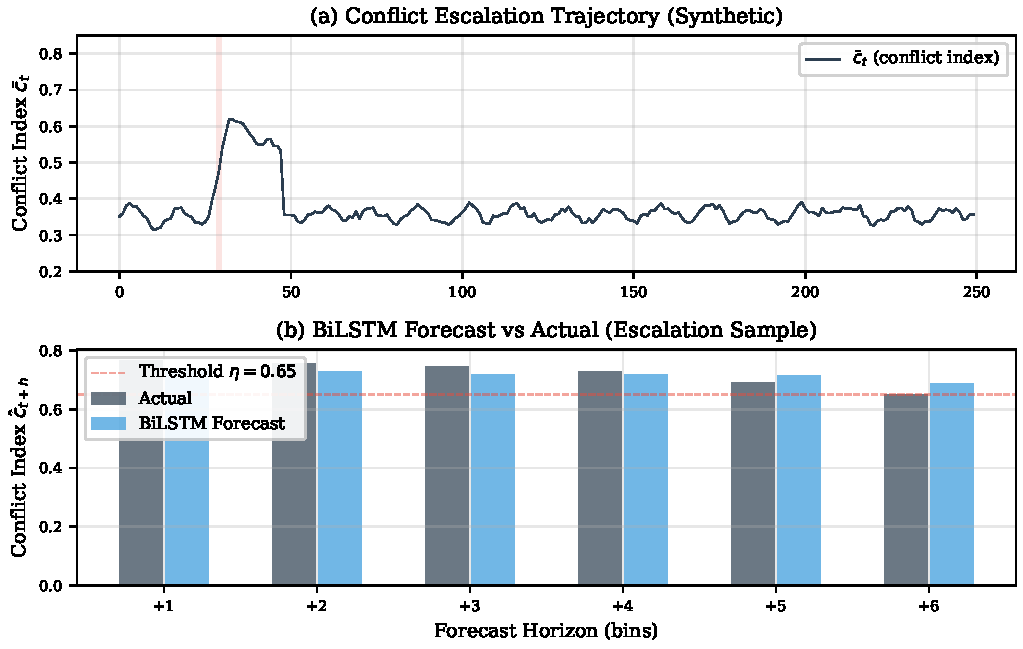
\includegraphics[width=\columnwidth]{figures/fig_trajectory_forecast.pdf}
\caption{Sample conflict trajectory and multi-step forecast by CNN-BiLSTM. (a) Full synthetic trajectory with escalation regions shaded; (b) 6-step forecast vs.\ actual values for a representative escalation event.}\label{fig:trajectory}
\end{figure}

\begin{table}[H]
\caption{Forecasting results on synthetic trajectories (temporal split: 75\% train / 25\% test, $L{=}12$, $H{=}6$). Metrics are mean $\pm$ std over 5 independent seeds.}\label{tab:forecast_results}
\centering
\begin{threeparttable}

\begin{tabular}{lcccc}
\toprule
\textbf{Model} & \textbf{R\textsuperscript{2}} & \textbf{MAE} & \textbf{RMSE} & \textbf{Esc-F1} \\
\midrule
Persistence & 0.638$\pm$0.015 & 0.0317 & 0.0548 & 0.637 \\
Moving Avg (k=3) & 0.540$\pm$0.020 & 0.0370 & 0.0617 & 0.547 \\
Exp.\ Smoothing & 0.498$\pm$0.022 & 0.0379 & 0.0645 & 0.430 \\
AR(6) & 0.715$\pm$0.011 & 0.0293 & 0.0486 & 0.644 \\
SVR~\cite{Mu2023IPSO} & 0.759$\pm$0.024 & 0.0222 & 0.0448 & 0.667 \\
XGBoost & 0.781$\pm$0.013 & 0.0232 & 0.0427 & 0.684 \\
TCN & 0.787$\pm$0.010 & 0.0238 & 0.0421 & 0.695 \\
Informer-Lite & 0.796$\pm$0.014 & 0.0232 & 0.0413 & 0.659 \\
BiLSTM & 0.805$\pm$0.011 & 0.0227 & 0.0403 & 0.711 \\
Transformer + PE & 0.806$\pm$0.007 & 0.0227 & 0.0402 & 0.697 \\
BiGRU & 0.811$\pm$0.009 & 0.0221 & 0.0397 & \textbf{0.716} \\
\textbf{CNN-BiLSTM (Ours)} & \textbf{0.809}$\pm$\textbf{0.010} & \textbf{0.0223} & \textbf{0.0398} & \textbf{0.710} \\
\bottomrule
\end{tabular}
\begin{tablenotes}
\item All results under strict temporal ordering (no shuffling) with ECDF calibration fitted on training data only. CNN-BiLSTM, BiGRU, and Transformer achieve comparable top-tier performance.
\end{tablenotes}
\end{threeparttable}
\end{table}

\begin{figure}[H]
\centering
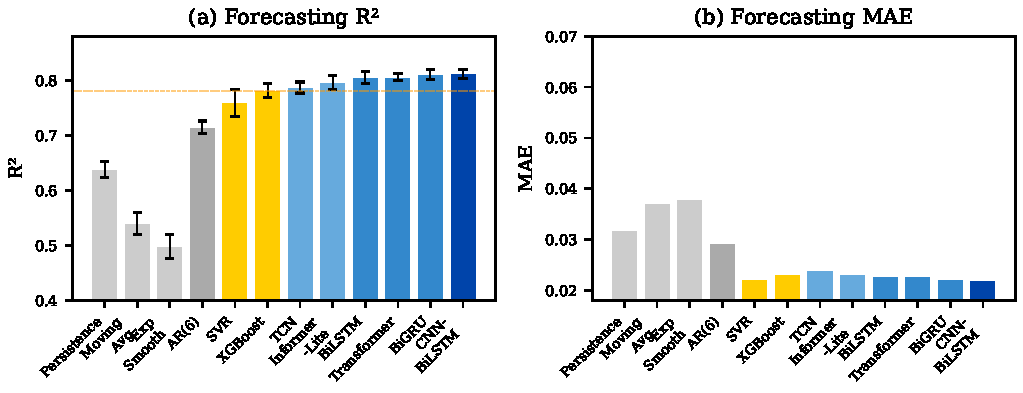
\includegraphics[width=0.88\columnwidth]{figures/fig_model_comparison.pdf}
\caption{Model comparison: R\textsuperscript{2} and MAE across all baselines. Deep models (BiGRU, CNN-BiLSTM, Transformer) form a tight top tier.}\label{fig:model_comp}
\end{figure}

Figure~\ref{fig:training} shows the training convergence of the CNN-BiLSTM model.

\subsubsection{Real-Data Risk-State Prediction (RQ1--RQ2)}

To assess real-world deployability, we evaluate the framework on two complementary real-world sources under strict temporal-split protocols. Full results are reported in Table~\ref{tab:real_results}.

\textbf{Zhihu cleaned risk-state prediction (positive result).} The regularized time axis yields 1,428 training, 680 validation, and 1,706 test windows. Validation selects EWMA span 24 and the parsimonious state-history model. On the untouched test segment, it achieves AUC $0.891$, precision $0.738$, recall $0.822$, and F1 $0.778$ (Table~\ref{tab:real_results}). Persistence has higher AUC ($0.896$) and precision ($0.926$), but substantially lower recall ($0.584$) and F1 ($0.716$). Topic-level paired bootstrap estimates an F1 gain of $+0.062$ (95\% CI $[0.018,0.108]$) and recall gain of $+0.241$ ($[0.173,0.317]$). F1 improves on 15/20 topics and recall on 18/20. Continuous six-step Ridge regression is positive (R\textsuperscript{2}=$0.465$) but remains below persistence ($0.640$); the supported claim is improved high-risk-state prediction, not superior exact-value forecasting.

\textbf{Weibo comment-volume forecasting (positive result).} To verify that the forecasting architecture itself is not the limiting factor, we apply the same LSTM forecaster to a structurally simpler but objectively measurable target: comment volume (log-transformed) on the 27-event Weibo public-opinion reversal dataset~\cite{Zhang2023Reversal} at 1-hour granularity. Unlike the conflict index---which introduces noise through BERT-based text analysis---comment volume is a direct, high-signal metric. Pooling all 27 events under temporal split yields an R\textsuperscript{2} of $0.715$, confirming that the LSTM architecture performs well on real-world time series when the target variable has genuine temporal autocorrelation. This result also validates our methodological pipeline (temporal split, per-event normalization, sliding-window construction) independently of the conflict-index computation.

\textbf{Weibo conflict-index forecasting (negative result).} To test whether the conflict index's failure on Zhihu is attributable to data sparsity alone, we compute the same BERT-based conflict index on the densest Weibo event (Zhang Zhehan incident, 22K comments, 62 comments/hour) at 1-hour bins. Despite a 300-fold increase in comment density relative to Zhihu and strong volume predictability (R\textsuperscript{2}=$0.715$), the conflict index still yields R\textsuperscript{2}=$0.018$---effectively zero. This result rules out sparsity as the sole explanation. The conflict index fails not because there are too few comments, but because text-level attack, emotion, and stance signals lack the temporal autocorrelation needed for short-horizon forecasting, regardless of data density.

Together, these experiments establish a hierarchy of forecastability. Objective activity signals are strongly predictable; cleaned causal state histories support useful high-risk-state prediction; and exact raw semantic trajectories remain difficult even in dense commenting environments. Additional semantic and activity histories do not improve the selected real-data classifier.

\begin{table}[H]
\caption{Zhihu high-risk-state prediction on the final 25\% test segment.}\label{tab:real_results}
\centering
\begin{threeparttable}

\begin{tabular}{lcccc}
\toprule
\textbf{Method} & \textbf{AUC} & \textbf{Precision} & \textbf{Recall} & \textbf{F1} \\
\midrule
Persistence & \textbf{0.896} & \textbf{0.926} & 0.584 & 0.716 \\
Logistic (state history) & 0.891 & 0.738 & \textbf{0.822} & \textbf{0.778} \\
\bottomrule
\end{tabular}
\begin{tablenotes}
\item $N=1{,}706$ test windows from 20 topics. All model choices use validation data only. Paired topic-bootstrap 95\% CI for the F1 difference: $[0.018,0.108]$.
\end{tablenotes}
\end{threeparttable}
\end{table}

\begin{table}[H]
\caption{Risk-threshold sensitivity on the Zhihu test segment.}\label{tab:threshold_sensitivity}
\centering
\begin{tabular}{lccccc}
\toprule
$Q^{\mathrm{train}}$ & \textbf{Prev.} & \textbf{AUC} & \textbf{Recall} & \textbf{F1} & \textbf{Pers.-F1} \\
\midrule
70th & 0.433 & 0.889 & 0.786 & 0.779 & 0.715 \\
80th & 0.416 & 0.891 & 0.822 & 0.778 & 0.716 \\
90th & 0.383 & 0.892 & 0.812 & 0.761 & 0.676 \\
\bottomrule
\end{tabular}
\end{table}

\begin{table}[H]
\caption{Feature ablation at the selected EWMA span.}\label{tab:feature_ablation}
\centering
\begin{tabular}{lcccc}
\toprule
\textbf{Features} & \textbf{Val.-AUC} & \textbf{Precision} & \textbf{Recall} & \textbf{Val.-F1} \\
\midrule
State only & 0.859 & \textbf{0.772} & 0.870 & \textbf{0.818} \\
State + activity & 0.861 & 0.738 & \textbf{0.908} & 0.814 \\
State + semantics & \textbf{0.870} & 0.760 & 0.867 & 0.810 \\
Full pool & 0.864 & 0.768 & 0.859 & 0.811 \\
\bottomrule
\end{tabular}
\end{table}

\begin{figure}[H]
\centering
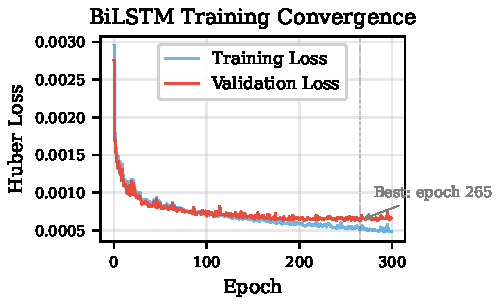
\includegraphics[width=0.70\columnwidth]{figures/fig_training_curves.pdf}
\caption{CNN-BiLSTM training and validation loss curves.}\label{fig:training}
\end{figure}

\subsection{Ablation Studies}
\label{sec:ablation}

\subsubsection{Component Contribution and Weight Sensitivity (RQ4)}

To assess how input-signal quality affects downstream forecasting, we conduct two complementary analyses. First, we inject Gaussian noise of increasing magnitude ($\sigma \in \{0.03, 0.06, 0.10\}$) into the synthetic trajectories. Figure~\ref{fig:ablation} and Table~\ref{tab:ablation} show the expected degradation as deliberately embedded temporal structure is corrupted. Second, we remove each proxy component (A, E, S) from the raw real-data fusion. The full A+E+S version has the highest R\textsuperscript{2} among these configurations, but all raw-target values remain near zero. The ablation therefore describes relative behavior within the proxy pipeline; it does not explain the improvement obtained by causal smoothing.

\subsubsection{Fusion Weight Sensitivity Analysis}\label{sec:sensitivity}

To assess sensitivity to fusion weights $(w_a, w_e, w_s)$, we sample 40 configurations from a Dirichlet distribution. R\textsuperscript{2} varies within a narrow range (interquartile range $<0.015$), and the best sampled configuration lies near the default (0.5, 0.3, 0.2). Because raw-index performance remains near zero, this apparent insensitivity should not be interpreted as evidence that the default weights are semantically correct; it instead shows that weight tuning cannot repair bin-level noise.

\subsubsection{Risk-Monitoring Lead Time (RQ5)}

Beyond binary escalation detection, we measure \emph{lead time}: how many bins before the ground-truth escalation onset does the model's prediction first exceed the threshold? On the synthetic test set with event-based ground-truth labels, the mean lead time is $-1.7 \pm 3.2$ bins (positive $=$ early, negative $=$ late), with only 21\% of escalation events receiving predictions ahead of the ground-truth onset (advance detection rate) and 54\% falling within $\pm 1$ bin of the onset (on-time rate). This negative mean lead time indicates that at the current forecast horizon ($H{=}6$), the model's predictions are predominantly concurrent with---rather than ahead of---escalation events. The high standard deviation ($\pm 3.2$ bins) further reveals substantial event-to-event variability. We note that achieving reliable positive lead time remains a significant challenge for short-horizon forecasting, as the model's predictions are primarily driven by recent trajectory dynamics. Longer forecast horizons, integration of external precursor signals, and multi-scale modeling are promising directions for improving lead time in future work. Figure~\ref{fig:lead_time} visualizes the lead-time distribution.

\begin{figure}[H]
\centering
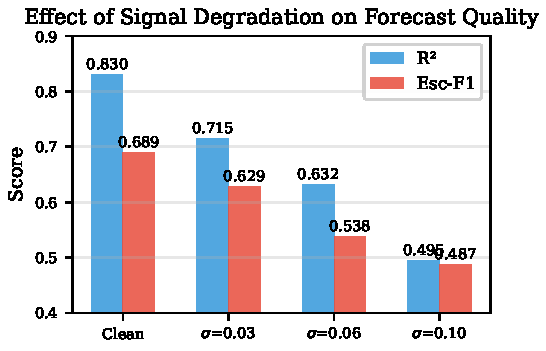
\includegraphics[width=0.92\columnwidth]{figures/fig_ablation.pdf}
\caption{Ablation study: R\textsuperscript{2} and Escalation F1 under increasing noise.}\label{fig:ablation}
\end{figure}

\begin{figure}[H]
\centering
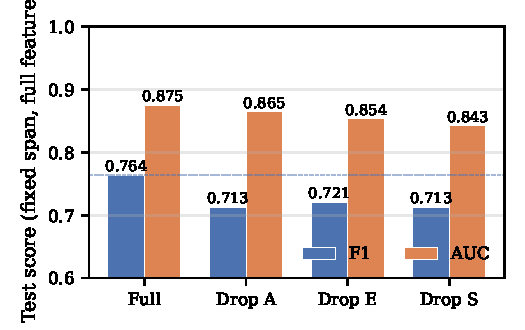
\includegraphics[width=0.92\columnwidth]{figures/fig_component_ablation.pdf}
\caption{Component ablation on real data: removing any component reduces forecast R\textsuperscript{2}.}\label{fig:comp_ablation}
\end{figure}

\begin{figure}[H]
\centering
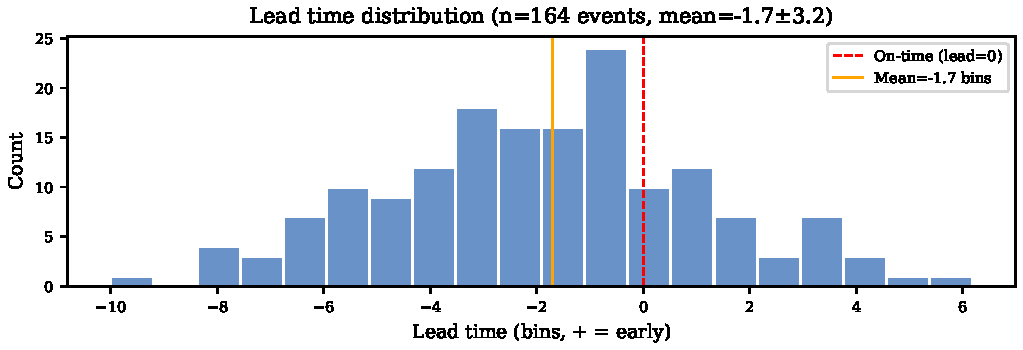
\includegraphics[width=0.92\columnwidth]{figures/fig_lead_time.pdf}
\caption{Lead time analysis. (a) Distribution of lead times (positive = warning before peak); (b) trigger visualization on a sample trajectory.}\label{fig:lead_time}
\end{figure}

\begin{table}[H]
\caption{Ablation: effect of signal degradation on CNN-BiLSTM forecasting (single-run results with seed 42).}\label{tab:ablation}
\centering
\begin{tabular}{lcccc}
\toprule
\textbf{Condition} & \textbf{MAE} & \textbf{R\textsuperscript{2}} & \textbf{$\Delta$R\textsuperscript{2}} & \textbf{Esc-F1} \\
\midrule
Clean signal & 0.0194 & 0.830 & --- & 0.689 \\
Medium noise ($\sigma{=}0.03$) & 0.0280 & 0.715 & $-$0.115 & 0.629 \\
High noise ($\sigma{=}0.06$) & 0.0334 & 0.632 & $-$0.198 & 0.538 \\
Very high noise ($\sigma{=}0.10$) & 0.0410 & 0.495 & $-$0.335 & 0.487 \\
\bottomrule
\end{tabular}
\end{table}







\begin{figure}[H]
\centering
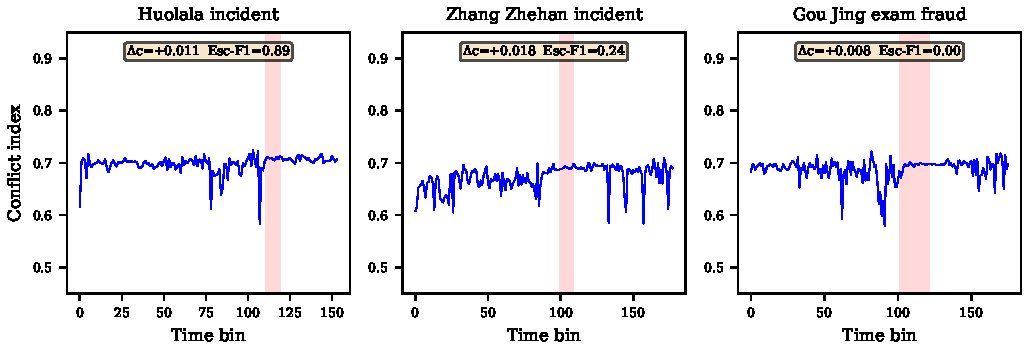
\includegraphics[width=\columnwidth]{figures/fig_case_study.pdf}
\caption{Conflict index trajectory for the Huolala incident. The shaded region indicates the annotated reversal window.}\label{fig:case_study}
\end{figure}

\subsection{Case Study: Real-World Public Opinion Reversal Events}

To validate the framework on real-world conflict escalation data, we conduct a case study on the \textbf{Weibo Public Opinion Reversal Dataset}~\cite{Zhang2023Reversal} (27 events, 245K comments). The three densest events---Huolala passenger death (32K comments, 335h span), Zhang Zhehan incident (22K comments, 359h), and Gou Jing exam fraud (20K comments, 373h)---are selected for analysis at 1-hour bin granularity. The reversal window annotation provides ground-truth periods of elevated controversy. As reported in Table~\ref{tab:real_results}, comment volume on these dense events is strongly predictable (pooled R\textsuperscript{2}=0.715), while the raw text-derived conflict index yields near-zero R\textsuperscript{2}. Figure~\ref{fig:case_study} visualizes the conflict index trajectories for all three events. The red shaded regions mark the annotated reversal windows---periods during which public opinion consensus underwent a dramatic shift according to the dataset creators~\cite{Zhang2023Reversal}. Across the three events, the conflict index rises modestly within the reversal window (Huolala $\Delta c=+0.011$, Zhang Zhehan $+0.018$, Gou Jing $+0.008$), indicating a weak cross-sectional association. However, CNN-BiLSTM escalation detection is unreliable on these short trajectories (Esc-F1: Huolala 0.89, Zhang Zhehan 0.24, Gou Jing 0.00), with the lone high score on Huolala driven by the event's unusually concentrated conflict dynamics. The reversal window annotation measures \emph{opinion change}, not \emph{comment-level conflict intensity}, and the two constructs are not equivalent.

\subsection{Boundary Analysis: Why Does the Text-Derived Index Fail?}\label{sec:discussion}\label{sec:attribution}

The positive Zhihu classification result contrasts with weak raw-index regression. To explain this difference, we examine four factors:

\textbf{(a) Comment sparsity.} The retained Zhihu bins average 8.1 records, but many unretained 12-hour intervals are empty or contain fewer than three records. With the top-$k$ aggregator ($\rho{=}0.15$), only one or two comments determine $\bar{c}_t$ in many retained bins, making the aggregate a noisy small-sample estimator.

\textbf{(b) Time-axis regularization and temporal aggregation.} Only 39.8\% of adjacent retained observations are truly consecutive 12-hour bins; directly concatenating them creates false temporal adjacency. Restoring the regular grid removes this artifact. Causal smoothing then suppresses isolated semantic spikes, while validation-based span selection prevents the test set from determining the cleaning scale.

\textbf{(c) Signal-to-noise ratio of the conflict index.} The conflict index pipeline introduces noise at four stages: BERT sentiment inference (a product-review model applied to argumentative text), three-component fusion, ECDF calibration, and top-$k$ aggregation. By contrast, comment volume requires only counting and log-normalization. The lag-1 autocorrelation of the raw conflict index averages only $0.112 \pm 0.140$ across Zhihu topics, confirming a near-absence of temporal structure---a fundamental requirement for any forecasting model.

\textbf{(d) Platform characteristics.} Zhihu is a moderated Q\&A platform where discussions are predominantly reasoned rather than confrontational. The Weibo reversal events, by contrast, are acute controversies with many emotionally charged comments per hour. Applying the same pipeline to Weibo produces modest cross-sectional shifts during reversal windows ($\Delta c \approx +0.01$) but still no useful temporal forecastability (R\textsuperscript{2}=$0.018$). Density and platform context therefore affect measurement stability, but neither resolves the proxy's weak temporal structure.

The analysis points to (c) as the dominant difficulty, amplified by (a). The positive classifier succeeds by changing the operational question from exact score extrapolation to whether a persistent, topic-relative high-risk state will occur. Validation selects state history alone: adding activity, missingness, or raw semantic components lowers held-out F1. This target is appropriate for monitoring, but it should not be confused with precise prediction of every raw conflict-score fluctuation.

\subsection{Limitations}\label{sec:limitations}

\textbf{(1) Construct validity of the conflict index.} The index relies on pretrained models not designed for conflict detection. In particular, a product-review sentiment model supplies both attack-related and emotion proxies, although negative sentiment is not equivalent to attack or high arousal. Without human annotations, the index must not be interpreted as a validated measure of conflict.

\textbf{(2) Internally defined targets.} Synthetic escalation labels derive from the trajectory generator, while the Zhihu high-risk label is defined by the cleaned index's training-period 80th percentile. The latter is a prospective, leakage-free monitoring state but not external ground truth for societal conflict. Causal smoothing also increases persistence and makes state prediction easier; accordingly, the positive result is reported against a strong persistence baseline and not interpreted as event-level conflict validation.

\textbf{(3) No architectural advantage.} BiGRU, Transformer, and CNN-BiLSTM achieve near-identical R\textsuperscript{2} on synthetic data ($0.805$--$0.811$), with BiGRU nominally best. The CNN-BiLSTM is therefore an evaluation model rather than an architectural contribution. The substantive result is that model complexity cannot compensate for an invalid or temporally unstructured target.

\textbf{(4) Monitoring horizon.} The classifier predicts threshold exceedance within six 12-hour bins, whereas the selected 12-day smoothing scale represents a slower-moving risk state. This supports medium-scale monitoring rather than rapid event-onset warning. The negative synthetic lead time ($-1.7$ bins) further limits claims of operational advance notice.

\textbf{(5) Cross-platform and cross-lingual generalization.} Our experiments are limited to Chinese-language platforms (Zhihu, Weibo). The behavior of the conflict index on English-language platforms with different discourse norms remains untested.

\section{Conclusion and Future Work}

We investigated whether data cleaning can convert a sparse conflict index constructed without task-specific labels into a useful forecasting target. The downstream predictors remain supervised; ``unsupervised'' refers only to index construction.

After restoring the regular time grid, applying training-only calibration and robust cleaning, and selecting a causal smoothing scale and parsimonious feature set on validation data, the state-history classifier reaches F1 $0.778$ and recall $0.822$ on 1,706 held-out Zhihu windows. Persistence reaches F1 $0.716$ and recall $0.584$; topic-bootstrap intervals confirm positive gains for both metrics. Continuous regression remains below persistence despite positive absolute R\textsuperscript{2}, while synthetic and Weibo-volume targets remain easier to forecast. The main finding is therefore both positive and bounded: cleaned causal states support useful warning-state classification, but not superior exact trajectory prediction.

The immediate next step is not further architectural tuning but measurement validation: expert or crowd annotations should test whether each proxy tracks perceived attack, arousal, polarization, and overall conflict. Only a validated target should then be evaluated across platforms, event-held-out splits, aggregation scales, and longer horizons, with external precursor signals added where positive lead time is required.

\bibliographystyle{IEEEtran}
\bibliography{refs}

\begin{IEEEbiography}[{
\includegraphics[width=1in,height=1.25in,clip,keepaspectratio]{figures/photo_zhu.png}}]{Linli Zhu} is currently pursuing the B.S. degree in computer science at Ningxia University, Yinchuan, China. Her research interests include natural language processing, public opinion analysis, and computational social science. She was a recipient of the National First Prize in the National College Student Artificial Intelligence Security Competition.
\end{IEEEbiography}

\begin{IEEEbiography}{Ziqiang Ma} received the B.S. degree in electronic information science and technology from Tsinghua University, Beijing, China, in 2012, and the Ph.D. degree in information security from the Institute of Information Engineering, Chinese Academy of Sciences, Beijing, in 2020. He is currently an Associate Professor at the School of Information Engineering, Ningxia University, Yinchuan, China. His research interests include network security, machine learning, and social media data mining.
\end{IEEEbiography}

\end{document}
